\begin{tcolorbox}
	\vspace{60pt}
	\part{Appendices}
	\lettrine{W}{ith} over 39\,km of explored passage, \passage{Sistem Migovec} is the longest cave system in Slovenia, and ranks among the 100 longest worldwide, a remarkable feat after more forty years of dedicated expeditions. The description of every metre of this cave is impossible as countless recesses, cracks, indomitable crawls or squeezes saw the light of one or two cavers, who, running low on energy and motivation, decided that `that was it'. 

	Such passages may not be visited again in years, or indeed ever, as focus shifts towards other `leads', and will remain intact, but for the single track of footprints that bears witness to the presence of one explorer. Such passages may endure within memory as traces on a larger map or a name in a directory. Others will become highways, passed by many explorers en route to the business end of the cave: pitches, galleries, streamways, they bear the mark of our presence: footprints, dislodged boulders, ropes. 
	
	\mydelimiter

	In the following section of the book, we aim first to give an account of the geology of the mountain, explain our surveying technique and finally describe such routes which through their connections and their loops form the still growing skeleton of the system. The itineraries reported in the last chapter of this part range from short half-day trips  to longer excursions and through-trips and finally, navigation to the pushing fronts from the underground camps.
\end{tcolorbox}

	\backgroundsetup{	scale=1,
					color=black,
					opacity=1,
					angle=0,
					contents={%
							  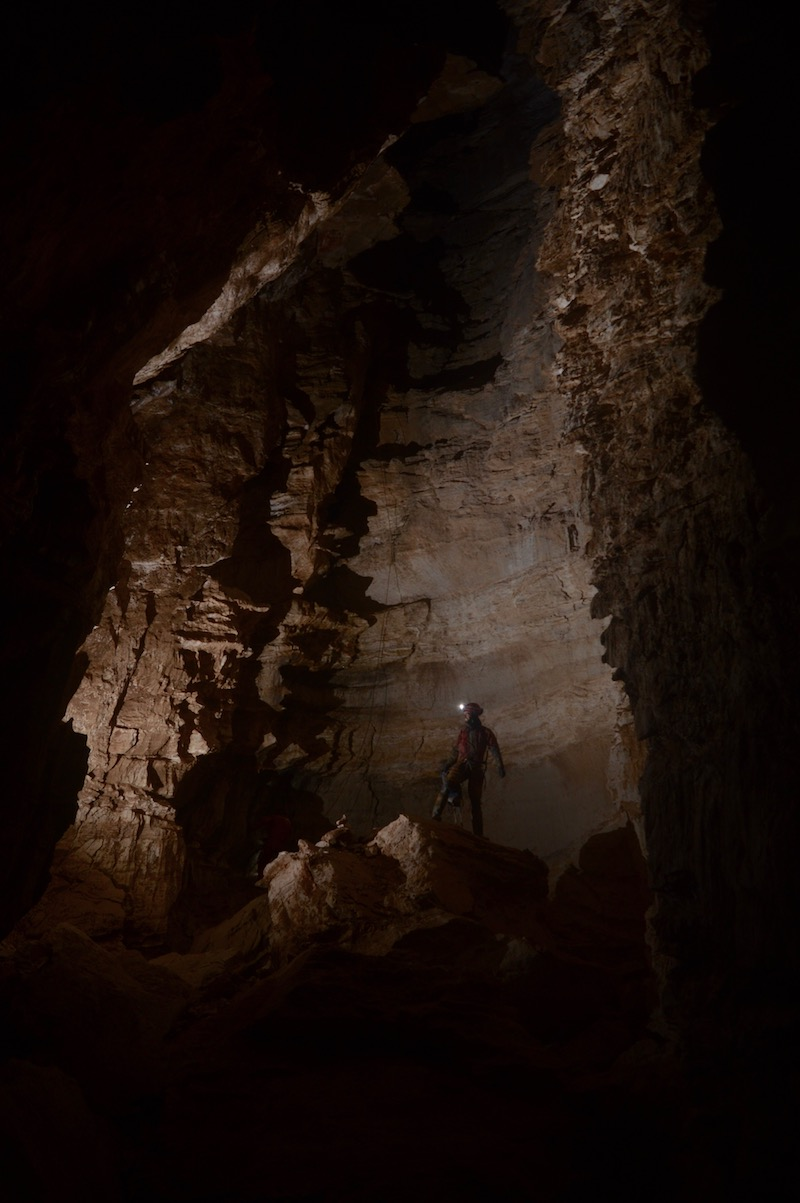
\includegraphics[width=\paperwidth]{images/backgrounds/jack-mountain-king.jpg}
  					}
	}
	
\BgThispage
